\documentclass[11pt]{standalone}
\usepackage{amssymb}
\usepackage{amsmath}
\usepackage[no-math]{fontspec}
\usepackage{unicode-math}
\usepackage{libertinus}
\usepackage{pgf,xcolor}
\usepackage{tikz}
\usetikzlibrary{arrows.meta, backgrounds, calc}
\usepackage{pgfplots}
\pgfplotsset{compat=newest}

% ── Color palette (all seven defined in every file) ──────────────────────────
\definecolor{my_darkgray}{HTML}{484949}
\definecolor{my_lightgray}{HTML}{F3F4F4}
\definecolor{my_darkblue}{HTML}{005A94}
\definecolor{my_lightblue}{HTML}{CCDEE9}
\definecolor{my_yellow}{HTML}{FFEC7F}
\definecolor{my_red}{HTML}{E60000}
\definecolor{my_orange}{HTML}{E87846}

\begin{document}
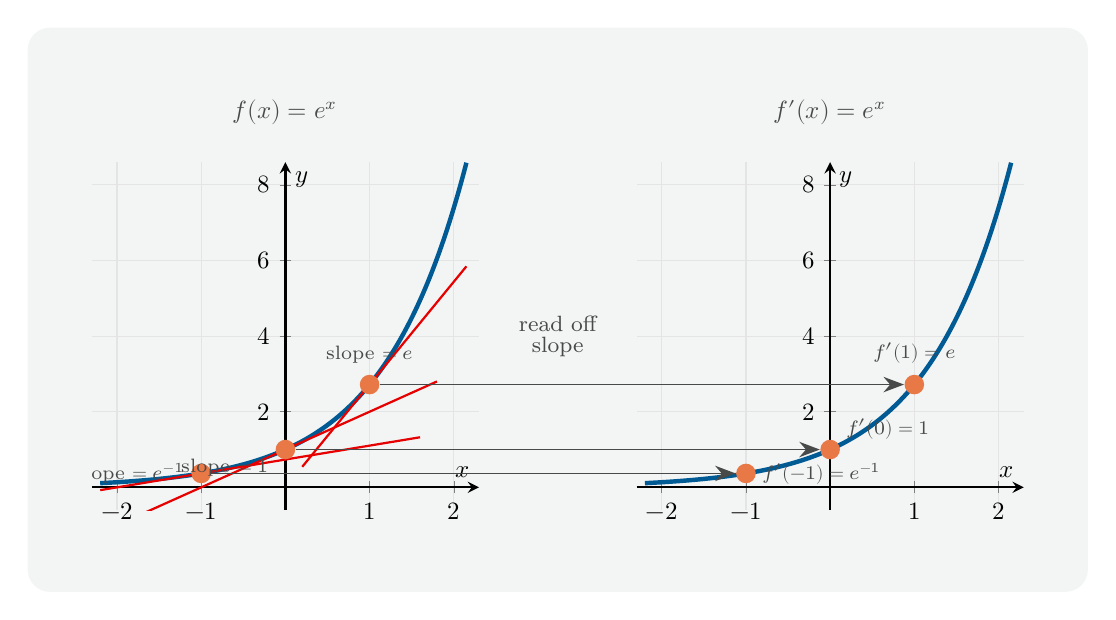
\begin{tikzpicture}[
    show background rectangle,
    background rectangle/.style={fill=my_lightgray, rounded corners=8pt},
    inner frame sep=0.8cm
]

% ── Left panel: f(x) = e^x with tangent lines at x = -1, 0, 1 ───────────────
%
% axis equal omitted: y range [0, 8] against x range [-2, 2] would produce
% an unreadably tall panel at equal scale.
%
\begin{axis}[
    name             = ax_left,
    width            = 6.5cm,
    height           = 6.0cm,
    axis lines       = center,
    xlabel           = {$x$},
    ylabel           = {$y$},
    grid             = both,
    grid style       = {color=my_darkgray!15},
    xmin = -2.3,  xmax = 2.3,
    ymin = -0.6,  ymax = 8.6,
    axis line style  = {thick},
    title            = {$f(x) = e^x$},
    title style      = {font=\small\bfseries, color=my_darkgray, yshift=4pt},
    tick label style = {font=\small},
    label style      = {font=\small},
    xtick            = {-2,-1,0,1,2},
    ytick            = {0,2,4,6,8},
]

  % Primary curve
  \addplot[color=my_darkblue, samples=300, ultra thick,
           domain=-2.2:2.15]{exp(x)};

  % Tangent at x=-1: slope = e^{-1}, passes through (-1, e^{-1})
  %   y = e^{-1}(x+2)
  \addplot[color=my_red, thick, domain=-2.2:1.6]{exp(-1)*(x+2)};

  % Tangent at x=0: slope = 1, passes through (0,1)
  %   y = x+1
  \addplot[color=my_red, thick, domain=-2.2:1.8]{x+1};

  % Tangent at x=1: slope = e, passes through (1, e)
  %   y = e*x
  \addplot[color=my_red, thick, domain=0.2:2.15]{exp(1)*x};

  % ── Sample point markers (also serve as named export nodes) ─────────────
  % The node names L1, L2, L3 are accessible in the outer tikzpicture.
  \node[circle, fill=my_orange, inner sep=2.5pt] (L1)
      at (axis cs:-1, {exp(-1)}) {};
  \node[circle, fill=my_orange, inner sep=2.5pt] (L2)
      at (axis cs:0,  1) {};
  \node[circle, fill=my_orange, inner sep=2.5pt] (L3)
      at (axis cs:1,  {exp(1)}) {};

  % ── Slope annotations to the left of each tangent point ─────────────────
  \node[font=\scriptsize, color=my_darkgray, anchor=east]
      at (axis cs:-1.08, {exp(-1)})
      {slope $= e^{-1}$};
  \node[font=\scriptsize, color=my_darkgray, anchor=north east]
      at (axis cs:-0.08, 1.0)
      {slope $= 1$};
  \node[font=\scriptsize, color=my_darkgray, anchor=south]
      at (axis cs:1.0, {exp(1)+0.3})
      {slope $= e$};

\end{axis}

% ── Right panel: f'(x) = e^x ─────────────────────────────────────────────────
\begin{axis}[
    name             = ax_right,
    at               = {(ax_left.east)},
    anchor           = west,
    xshift           = 2.0cm,
    width            = 6.5cm,
    height           = 6.0cm,
    axis lines       = center,
    xlabel           = {$x$},
    ylabel           = {$y$},
    grid             = both,
    grid style       = {color=my_darkgray!15},
    xmin = -2.3,  xmax = 2.3,
    ymin = -0.6,  ymax = 8.6,
    axis line style  = {thick},
    title            = {$f'(x) = e^x$},
    title style      = {font=\small\bfseries, color=my_darkgray, yshift=4pt},
    tick label style = {font=\small},
    label style      = {font=\small},
    xtick            = {-2,-1,0,1,2},
    ytick            = {0,2,4,6,8},
]

  % Derivative curve (identical to f — this is the key observation)
  \addplot[color=my_darkblue, samples=300, ultra thick,
           domain=-2.2:2.15]{exp(x)};

  % ── Derivative value markers ──────────────────────────────────────────────
  % Node names R1, R2, R3 are accessible in the outer tikzpicture.
  \node[circle, fill=my_orange, inner sep=2.5pt] (R1)
      at (axis cs:-1, {exp(-1)}) {};
  \node[circle, fill=my_orange, inner sep=2.5pt] (R2)
      at (axis cs:0,  1) {};
  \node[circle, fill=my_orange, inner sep=2.5pt] (R3)
      at (axis cs:1,  {exp(1)}) {};

  % ── Derivative value annotations to the right of each point ─────────────
  \node[font=\scriptsize, color=my_darkgray, anchor=west]
      at (axis cs:-0.92, {exp(-1)})
      {$f'(-1) = e^{-1}$};
  \node[font=\scriptsize, color=my_darkgray, anchor=south west]
      at (axis cs:0.08, 1.0)
      {$f'(0) = 1$};
  \node[font=\scriptsize, color=my_darkgray, anchor=south]
      at (axis cs:1.0, {exp(1)+0.3})
      {$f'(1) = e$};

\end{axis}

% ── Arrows from sample points on left to derivative values on right ───────────
% Both axes share the same y-range and height, so corresponding points sit at
% the same canvas height and the arrows are horizontal.
\draw[-{Stealth[scale=1.3]}, color=my_darkgray, semithick]
    (L1) to[out=0, in=180] (R1);
\draw[-{Stealth[scale=1.3]}, color=my_darkgray, semithick]
    (L2) to[out=0, in=180] (R2);
\draw[-{Stealth[scale=1.3]}, color=my_darkgray, semithick]
    (L3) to[out=0, in=180] (R3);

% ── Label in the arrow gap ────────────────────────────────────────────────────
% Placed at the midpoint between the two axes, vertically centred.
\node[font=\footnotesize, color=my_darkgray, align=center]
    at ($(ax_left.east)!0.5!(ax_right.west)$)
    {read off\\[-2pt]slope};

\end{tikzpicture}
\end{document}
